\documentclass{../../ktane-mod}
\RequirePackage{enumitem}

\setlength{\parindent}{0pt}
\setlength{\parskip}{10pt}

\begin{document}
\rhead{Modules}

\clearpage
% Start content at 1/3 from top of page
\vspace*{0.33\textheight}

% Center the content horizontally
\begin{center}
  \begin{minipage}{\textwidth}
    % Two-column layout with image on right, text on left
    \begin{minipage}[t]{0.65\textwidth}
      \setlength{\parskip}{10pt}
      \begin{center}
        \section*{Section 1: Modules}
        
        Modules can be identified by an LED in the top right corner.
        When this LED is lit green the module has been disarmed.

        All modules must be disarmed to defuse the bomb.
      \end{center}
    \end{minipage}%
    \hfill%
    \begin{minipage}[t]{0.3\textwidth}
      \centering
      \raisebox{\dimexpr\ht\strutbox+\dp\strutbox-\height}{%
        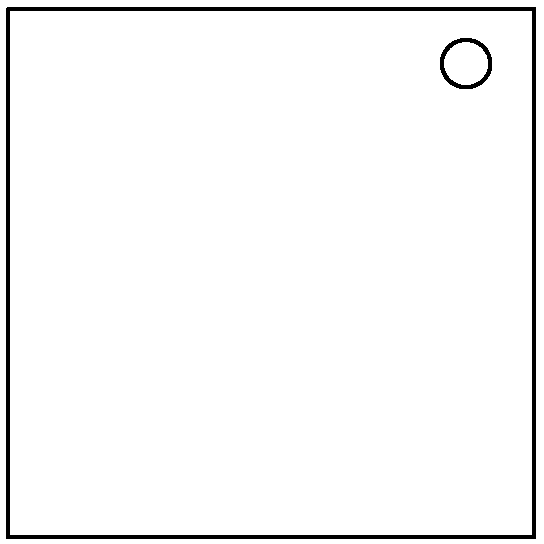
\includegraphics[height=3.5cm]{module_img}%
      }
    \end{minipage}
  \end{minipage}
\end{center}

\cleardoublepage
\end{document}
